\appendix

\chapter{Rotational Bands in Nuclei}
\label{appendix:ral-dal-signature-scheme}

Based on the behavior of $\mathbf{j}$ and its coupling with the collective angular momentum, two rotational rotational modes can occur. The two scenarios are \emph{Deformation aligned bands} and \emph{Rotation aligned bands} \cite{uwitonze2015assignment}, and the two modes will be described herein. A graphical representation with both rotational schemes can be seen in Fig. \ref{ral-dal-coupling-bands}.
\begin{figure}
    \centering
    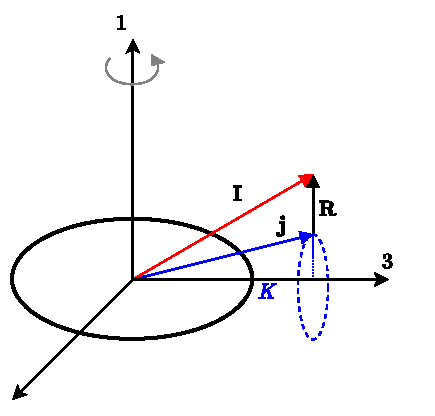
\includegraphics[width=0.49\textwidth]{Chapters/Figures/DAL_scheme.pdf}
    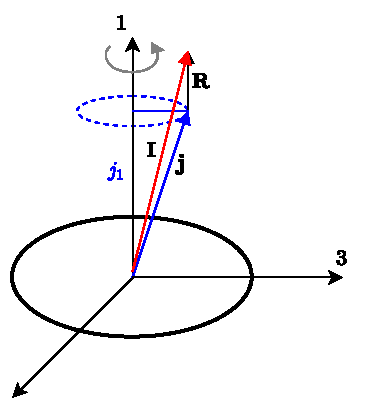
\includegraphics[width=0.49\textwidth]{Chapters/Figures/RAL_scheme.pdf}
    \caption{A sketch with the geometrical interpretation of the two ways a nucleus can exhibit rotational bands: Deformed Aligned Bands (\textbf{left}) and Rotation Aligned Bands (\textbf{right}). The projection of the single-particle's total a.m. on the deformation and rotation axes is denoted by $K$ and $j_1$, respectively.}
    \label{ral-dal-coupling-bands}
\end{figure}

\section{Deformation Aligned Bands}

This case is also known as \emph{strong-coupling limit} \cite{bohr1953collective}, since the particle's a.m. is tightly coupled to the deformation axis (i.e., the symmetry axis). The general Hamiltonian will be:
\begin{align}
    H_\text{rot}=H_0+H_\text{coupl}\ ,
\end{align}
where $H_0$ is the operator containing the squared components $I_k$ of $\mathbf{I}$ and the extra \emph{coupling term} represents the Coriolis force \cite{bertulani2007nuclear}. The Coriolis effect is reflected by the coupling of the collective motion of the nucleus to the odd nucleon's motion. Despite that, it can be neglected at small rotations. The projection of the particle's a.m. on the symmetry axis is a good quantum number and if $\mathbf{R}$ is pointing in a direction perpendicular to the deformation axis, then $\Omega=K$. Accordingly, the energy spectrum will be given by:
\begin{align}
    E_\text{rot}(I)=\frac{\hbar^2}{2\mathcal{I}_\perp}\left[I(I+1)-K(K+1)\right]\ ,
\end{align}
or more formally:
\begin{align}
    E_\text{rot}(I)=\frac{\hbar^2}{2\mathcal{I}_\perp}\left[I(I+1)-K^2\right]+E_0(K)\ .
\end{align}

The rotational band will be constructed on the ground-state $E_0(K)$, where the total spin $I$ will consist of a sequence $I=K,K+1,K+2,\dots$ having $K\neq 1/2$. Consequently, rotational bands will have consecutive states differing by only one unit of angular momentum. It should be pointed out that odd-$A$ nuclei can have multiple rotational bands built on different values of $K$. For $K=1/2$, the band structure will follow:
\begin{align}
    E_\text{rot}(I)=\frac{\hbar^2}{2\mathcal{I}_\perp}\left[I(I+1)+a(-)^{I+\frac{1}{2}}(I+\frac{1}{2})\right]\ .
    \label{deformation-aligned-energy}
\end{align}

The nature of $(-1)^{I+1/2}$ will be explained in the next section, which depicts the \emph{Rotation Aligned Bands}. Moreover, the term $a$ is called the \emph{decoupling parameter} \cite{bertulani2007nuclear}, and it can be determined from the first two experimental energy levels. Experimental data exhibiting rotational bands with $K=1/2$ and $K\neq 1/2$ are shown for two odd-$A$ nuclei in Fig. \ref{rotational-bands-odd-a}.
\begin{figure}
    \centering
    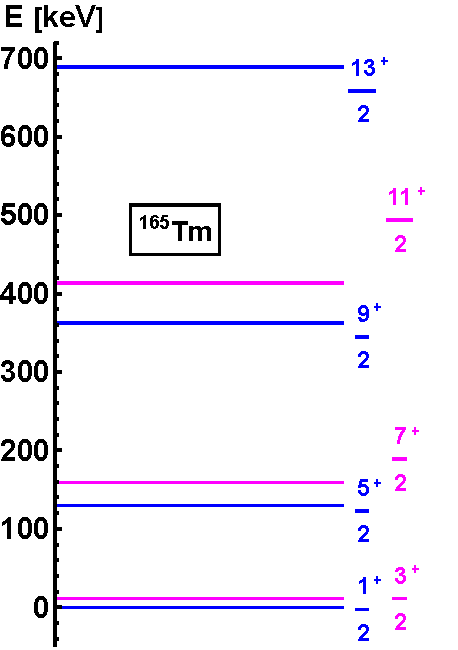
\includegraphics[scale=0.7]{Chapters/Figures/Tm165-Rotational-Bands.pdf}
    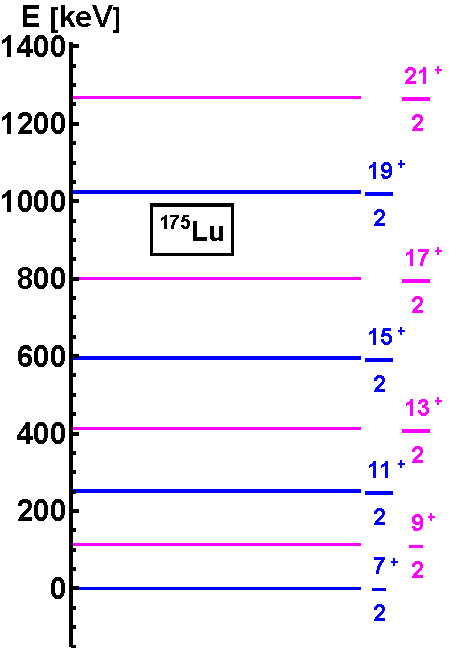
\includegraphics[scale=0.7]{Chapters/Figures/Lu175-Rotational-Bands.pdf}
    \caption{Rotational bands in odd-$A$ nuclei with the $K$ quantum number equal to $K=1/2$ (\textbf{left}) and $K\neq 1/2$ (\textbf{right}).}
    \label{rotational-bands-odd-a}
\end{figure}

\section{Rotation Aligned Bands}
\label{section-ral-signature}
This situation is also called the \emph{decoupling limit} \cite{bohr1998nuclear} and it leads to the apparition of \emph{decoupled bands}. Here the total angular momentum is more aligned with the axis of rotation, and its maximum projection is along this axis. This usually happens at high-spins, making the odd-particle's a.m. to tilt away from the symmetry axis and gradually align with the direction of rotation (via the Coriolis effect). As such, the coupling term $H_\text{coupl}$ from $H_\text{rot}$ is not neglected here:
\begin{align}
    H_\text{rot}=\frac{\hbar^2}{2\mathcal{I}_\perp}\left(\mathbf{I}^2+\mathbf{j}^2-2\mathbf{I}\cdot\mathbf{j}\right)\ .
\end{align}

It is usually preferred to work with the raising and lowering operators: $\mathbf{I}_\pm=\mathbf{I}_1\pm i \mathbf{I}_2$ (and similarly for $\mathbf{j}$), bringing $H_\text{rot}$ to the following expression:
\begin{align}
    H_\text{rot}&=\frac{\hbar^2}{2\mathcal{I}_\perp}\hat{I}^2+\frac{\hbar^2}{2\mathcal{I}_\perp}\hat{j}^2-\frac{\hbar^2}{\mathcal{I}_\perp}K^2+H_\text{Coriolis}\ ,\\
    H_\text{Coriolis}&=-\frac{\hbar^2}{2\mathcal{I}_\perp}(\mathbf{I}_+\mathbf{j}_-+\mathbf{I}_-\mathbf{j}_+)\ .
\end{align}

The Coriolis term mixes bands differing in the $K$ by one unit, effect that is negligible at high deformations and low spins, since the single-particle motion is tightly bound to the bulk nucleus. On the other hand, at very high rotations it becomes significant. Consequently, the Coriolis effect most probably occurs in prolate nuclei for an `almost empty' $j$-shell and oblate nuclei for an `almost full' $j$-shell. When the single-particle angular momentum is oriented with the direction of rotation, the projection of $\mathbf{j}$ can be denoted by $j_1$ (keeping a consistency with Fig. \ref{rotational-coupling-schematic}). The spectrum of the decoupled bands will be:
\begin{align}
    E_\text{rot}(I)=\text{const.}+\frac{\hbar^2}{2\mathcal{I}_\perp}(I-j_1)(I-j_1+1)\ ,
\end{align}
where the coupling terms have been encapsulated in $\text{const.}$. This leads to a spin sequence $I=j_1,j_1+2,j_1+4\cdots$, which differs from the previous case via the constant $2\hbar$ angular momentum difference of two consecutive levels.

In order to understand the terms $(-1)^{I+1/2}$ from Eq. \ref{deformation-aligned-energy}, it is required to describe the wave-function of the particle-core system. Indeed, using the specific quantum numbers $I,K,M$ with their meaning explained in Fig. \ref{rotational-coupling-schematic}, the wave-function will be written as a combination of rotational (the Wigner-$\mathcal{D}_{MK}^I$ functions) and single-particle components \cite{wang2007exotic,davydov1958rotational}:
\begin{align}
    \Psi_{MK}^I=\ket{IMK}=N\left[\phi_K \mathcal{D}_{MK}^I+(-)^{I+K}\phi_{-K}\mathcal{D}_{M-K}^I\right]\ ,
    \label{RAL-bands-wave-function}
\end{align}
where $N$ is the normalization constant, usually having the value $N=\sqrt{\frac{2I+1}{16\pi^2}}$. This linear combination of states with $K$ and $-K$ induces a degeneracy due to the invariance with respect to rotations by $\pi$ around the rotational axis \cite{frauendorf1997tilted,bohr1998nuclear}. The factor $(-)^{I+K}\equiv\alpha$ is called the \emph{signature} and it reflects wether a system is invariant or not to such an rotation. More precisely, the \emph{signature quantum number} for a state $I$ in an odd-$A$ nucleus is given as \cite{sun1994varied}:
\begin{align}
    \alpha_I=\frac{1}{2}(-)^{I-\frac{1}{2}}\ ,
    \label{signature-quantum-number}
\end{align}
which results in the favored states having $\alpha_\textbf{favored}=\frac{1}{2}$ and the unfavored states having $\alpha_\textbf{unfavored}=-\frac{1}{2}$.

Depending on the signature, the nuclear states are split in two sets: one that follows $I=K,K+2,K+4,\dots$ and $I=K+1,K+3,K+5,\dots$. This is the reason why for the decoupled bands, one can regard them as an `initial' rotational band $I,I+1,\dots$ that is `broken' apart in two sequences: one that is favored and one that is unfavored (opposite signatures). An example is the odd-$A$ nucleus where the favored bands have spins $I_\text{favored}=\frac{1}{2},\frac{5}{2},\frac{9}{2},\dots$ and their unfavored \emph{partner} bands have spins $I_\text{unfavored}=\frac{3}{2},\frac{7}{2},\frac{11}{2},\dots$, which are also known as \emph{signature partners}. In fact, taking a closer look at the rotational bands shown in Fig. \ref{rotational-bands-odd-a}, each consecutive level is a state with different signature, meaning that each `group' of colors classifies into a set of favored (blue) and unfavored (magenta) states. The concept of signature partners will be crucial for a developed formalism that aims at describing rotational motion of highly deformed nuclei. This is treated throughout Chapters \ref{chapter-6-aw1-formalism} and \ref{chapter-7-novel}.

This divided set of partner bands has some characteristics that can be observed throughout experimental measurements. Firstly, the splitting of the two branches implies that the favored states will generally have lower excitation energy than their unfavored partners. This is also proved by the expression of the rotor energy given in Eq. \ref{deformation-aligned-energy}, where the decoupling parameter will cause an upward (downward) shift in energy for states with $I=1/2,5/2,9/2,\dots$ ($I=3/2,7/2,11/2,\dots$) if $a$ is positive (negative). The experimental data from Fig. \ref{level-scheme-signature-splitting} shows how the favored partner lies lower with respect to its unfavored partner bands, each having the corresponding spin sequence $\Delta I=2$ for intraband states and $\Delta I=1$ for interband states. Such spectra are often met in the decay schemes for odd-mass nuclei where the rotational motion is governed by the core + particle coupling scheme.
\begin{figure}
    \centering
    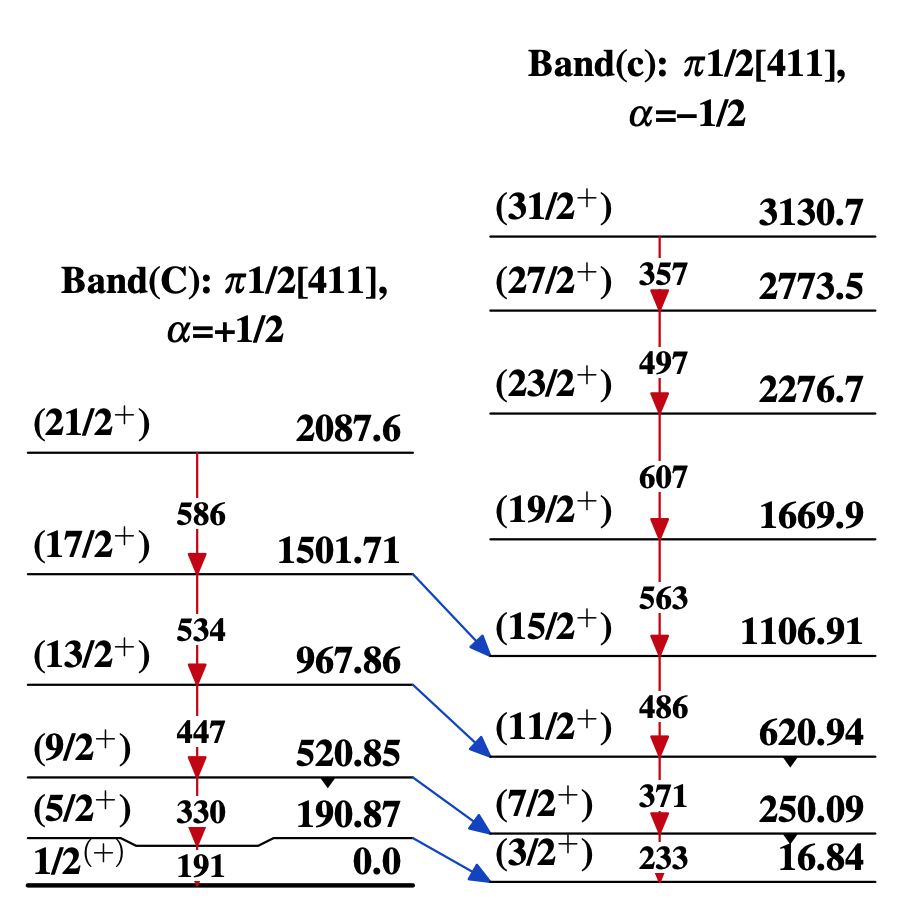
\includegraphics[width=0.38\textwidth]{Chapters/Figures/Lu_163_K12-band.png}
    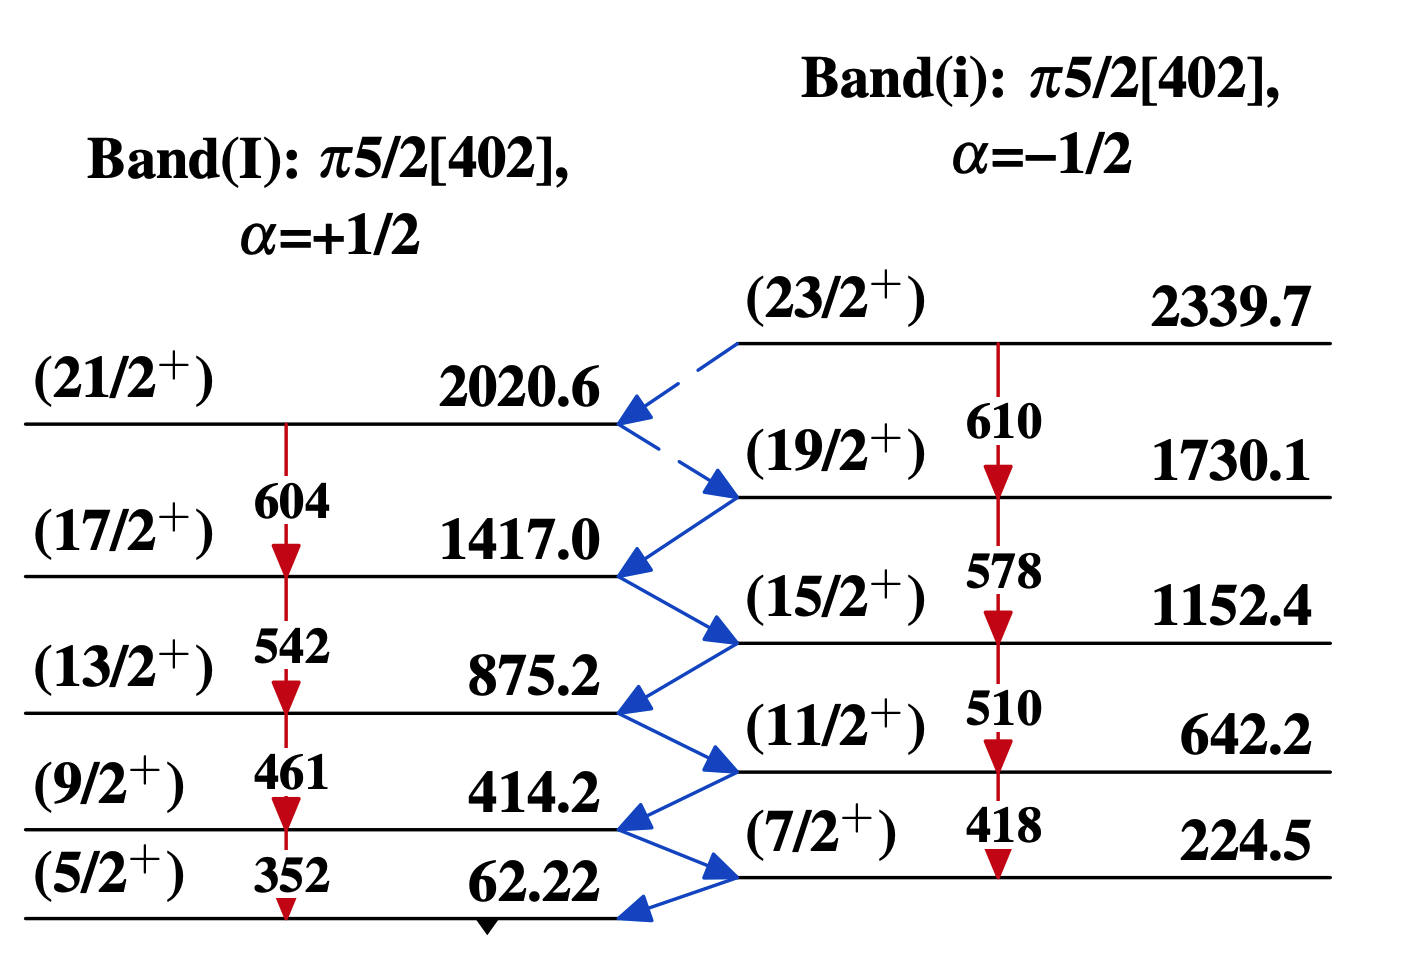
\includegraphics[width=0.38\textwidth]{Chapters/Figures/Lu_163_signatureSplitting.png}
    \caption{Experimental level schemes for $^{163}$Lu showing pairs of signature partner bands. \textbf{Left pair}: the two bands are built on a proton with $j=1/2$ and positive parity. \textbf{Right pair}: sequences built on a proton with $j=5/2$ with the same parity. The Nilsson quantum numbers are defined for each band. Note the lower energies for the favored states. Interband transitions are marked with the blue arrows. The experimental data is from Ref. \cite{reich2010nuclear} and the level schemes were taken from Ref. \cite{bhat1992evaluated}.}
    \label{level-scheme-signature-splitting}
\end{figure}
